\documentclass[border=4pt]{standalone}
\usepackage{amsmath,amssymb,amsfonts}
\usepackage{xcolor,colortbl,array,booktabs,multirow}
\usepackage{tikz}
\usepackage{pgfplots}
\pgfplotsset{compat=1.16}
\usetikzlibrary{arrows, automata, backgrounds, calendar, chains, decorations,
    matrix, mindmap, patterns, petri, positioning, shadows, shapes.geometric,
    trees, shapes, decorations.pathreplacing, calc, tikzmark, arrows.meta,
    intersections, fit, graphs, quotes, angles, decorations.markings}
\newcommand{\st}{\text{ s.t. }}
\newcommand{\x}{\mathbf{x}}
\renewcommand{\b}{\mathbf{b}}
\renewcommand{\c}{\mathbf{c}}
\newcommand{\A}{\mathbf{A}}
\newcommand{\y}{\mathbf{y}}
\newcommand{\z}{\mathbf{z}}
\newcommand{\R}{\mathbb{R}}
\newcommand{\RR}{\mathbb{R}}
\newcommand{\Z}{\mathbb{Z}}
\newcommand{\ZZ}{\mathbb{Z}}
\newcommand{\npcomplete}{NP-complete}
\providecommand{\true}{\text{TRUE}}
\providecommand{\false}{\text{FALSE}}
\tikzset{vertex/.style={circle,fill=black!25,minimum size=20pt,inner sep=0pt},
    edge/.style={draw,thick,-},weight/.style={font=\small},
    selected vertex/.style={vertex, fill=red!24},
    selected edge/.style={draw,line width=2pt,-,red!50},
    ignored edge/.style={draw,line width=2pt,-,black!20}}
\newcommand{\vect}{\vec}
\providecommand{\ds}{\displaystyle}
\providecommand{\longvect}{\overrightarrow}
\usepackage[normalem]{ulem}
\definecolor{ocre}{RGB}{243,102,25}
\providecommand{\leftB}{\left[}
\providecommand{\rightB}{\right]}
\tikzset{directed/.style={postaction={decorate,decoration={markings,mark=at position .65 with {\arrow{>}}}}},
    directed1/.style={postaction={decorate,decoration={markings,mark=at position .65 with {\arrow{>}}}}}}
\begin{document}
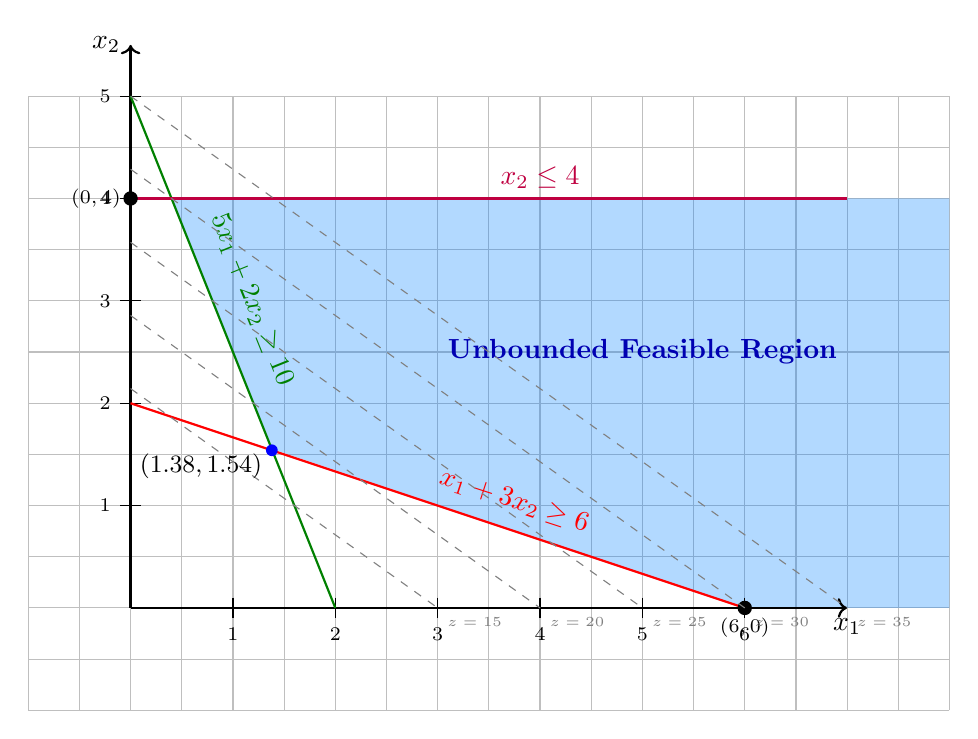
\begin{tikzpicture}[scale = 1.3]
    \draw[gray!50, thin, step=0.5] (-1,-1) grid (8,5);

    % Highlight the feasible region
    \fill[blue!50!cyan,opacity=0.3]
        (0.4,4) -- (1.39,1.55)  -- (6,0) -- (8,0) -- (8,4) -- cycle;

    % Define axes
    \draw[thick,->] (0,0) -- (7,0) node[anchor=north] {$x_1$};
    \draw[thick,->] (0,0) -- (0,5.5) node[anchor=east] {$x_2$};

    % Add tick marks on the x_1-axis
    \foreach \x in {1,2,3,4,5,6} {
        \draw (\x,0.1) -- (\x,-0.1) node[anchor=north] {\scriptsize $\x$};
    }

    % Add tick marks on the x_2-axis
    \foreach \y in {1,2,3,4,5} {
        \draw (0.1,\y) -- (-0.1,\y) node[anchor=east] {\scriptsize $\y$};
    }

    % Define the constraints
    % Line 1: X + 3Y = 6
    \draw[red,thick] (0,2) -- (6,0);
    \node[red, rotate=-18, anchor=north west] at (3,1.5) {$x_1 + 3x_2 \geq 6$};

    % Line 2: 5X + 2Y = 10
    \draw[green!50!black,thick] (0,5) -- (2,0);
    \node[green!50!black, rotate=-68, anchor=north west] at (1,4) {$5x_1 + 2x_2 \geq 10$};

    % Line 3: Y = 4
    \draw[purple,thick] (0,4) -- (7,4);
    \node[purple, rotate=0, anchor=south] at (4,4) {$x_2 \leq 4$};

    % Label feasible region
    \node[blue!70!black, font=\bfseries] at (5,2.5) {Unbounded Feasible Region};

    % Mark intersection points
\fill[black] (0,4) circle (2pt) node[anchor=east] {\scriptsize $(0,4)$};
\fill[black] (6,0) circle (2pt) node[anchor=north] {\scriptsize $(6,0)$};

% Objective function contours
\foreach \c in {15,20,25,30,35} {
    \draw[dashed,gray] (0,\c/7) -- (\c/5,0) node[below right] {\tiny$z = \c$};
    }
\node[blue,circle,fill,inner sep=1.5pt,label={[black,anchor=north east]\small$(1.38,1.54)$}] at (1.38,1.54) {};

\end{tikzpicture}
\end{document}
